\documentclass[10pt,a4paper,twocolumn]{article}
\usepackage[margin=2cm,columnsep=0.6cm]{geometry}
\usepackage[T1]{fontenc}
\usepackage{lmodern}
\usepackage{microtype}
\usepackage{graphicx}
\usepackage{booktabs}
\usepackage{enumitem}
\usepackage[font=small,labelfont=bf,skip=3pt]{caption}
\usepackage{titlesec}
\usepackage{xurl}
\usepackage[hidelinks]{hyperref}

\titleformat{\section}{\normalsize\bfseries}{}{0pt}{}
\titlespacing*{\section}{0pt}{6pt}{2pt}
\setlist{nosep,leftmargin=*}
\setlength{\parskip}{2pt}
\setlength{\parindent}{0pt}

\title{\vspace{-1.2cm}\Large Training a tumor-classifying CNN from scratch and compressing it to 1.4\,kB}
\author{Viktor Andri Hermannsson \\ \small Code: \url{https://github.com/Nussari/DNN-lok}}
\date{\vspace{-0.8cm}}

\begin{document}
\maketitle

The idea of shrinking models is exciting to me, so for this project I took the classic task of brain tumor
classification from MRI and added a twist: seeing how small I could get the model, and measuring the loss at
each step. I used BDNeuro-MRI v7~\cite{data} (CC BY 4.0), a pre-split dataset of labelled brain scans with three
tumor classes (glioma, meningioma, pituitary) and a ``no tumor'' class: 4,160 training, 892 validation and
889 test images.

The dataset authors list scores for seven models~\cite{bench}. I kept two as references: their CNN trained from
scratch (test accuracy 0.847) and the top performer, a fine-tuned ImageNet DenseNet121 (0.983). To start with, I
used the baseline of always choosing the largest class. That gave me a starting baseline, a ``realistic'' goal
and an optimistic goal.

\section{The data}
A few observations raised concerns when looking at the data:
\begin{enumerate}
  \item The data is skewed: the largest class is 2.78 times the size of the smallest.
  \item The data I thought was clean contained duplicates: 116 validation and test images were near-copies of
        training images. Removing them left a clean validation set (832) and clean test set (833).
  \item The no-tumor class contains a mix of scan types (T2, FLAIR, CT), whereas the tumor classes are almost
        all contrast-enhanced T1 MRI. That is a shortcut risk.
\end{enumerate}
The skew was kept in mind when selecting the metric and the duplicates were removed. The mix of scan types was not
addressed; instead it was kept in mind for possible image augmentation.

\section{Metrics and decisions}
\begin{itemize}
  \item \textbf{Balanced accuracy} was chosen as it best addresses the class imbalance. Several metrics were
        tested on ``dumb classifiers'' to see how they handle them.
  \item A set seed (1738) was chosen for reproducibility, but every option was trained with three seeds to
        guard against lucky seeds.
  \item As false negatives are worse than false positives, a model uses a cutoff on P(tumor) if its tumor
        sensitivity drops below 0.98 on the validation set. Only the smallest model ended up needing this.
\end{itemize}

\section{Pre-processing}
To feed the CNN a fixed input size, all images had to be brought to the same resolution. Three ways were tested:
\emph{stretch} the image, \emph{pad} the missing area, or \emph{crop} to the detected head area. Crop was picked,
as the tumorless class is mostly the one with varying image sizes and shapes, which raised the fear of models
learning ``stretched/padded means no tumor''.

\section{The ``large'' model}
I started with a sanity-check model to verify that labels, loss and data flow were wired correctly. Then,
starting from the majority-class baseline (balanced accuracy 0.25), I made a CNN (0.896 on validation) and
changed one thing at a time, keeping the model and its validation score as the new baseline whenever a change
beat it (Fig.~\ref{fig:progress}):
\begin{itemize}
  \item \textbf{First model:} early-stopping patience of 20 epochs.
  \item \textbf{Input:} per-image normalization, grayscale (over RGB), 128\,px.
  \item \textbf{Optimization:} Adam, learning rate 0.03, batch size 64, no schedule, label smoothing (which I
        later found out was a mistake).
  \item \textbf{Architecture:} 5x5 kernels, average pooling, BatchNorm kept. Smaller candidate: plain,
        5 layers, width 16. Deep candidate: residual, 17 layers, width 32.
  \item \textbf{Regularization:} mild augmentation, no weight decay, dropout only for the deep candidate (0.3).
\end{itemize}

\begin{figure}[t]
  \centering
  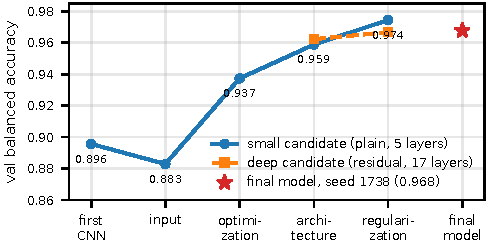
\includegraphics[width=\columnwidth]{fig_progress.pdf}
  \caption{Validation balanced accuracy (mean of 3 seeds) of the chosen model after each step. The input step dips because it was chosen on Apple M1 runs and retrained on the GPU.}
  \label{fig:progress}
\end{figure}

This left two candidates: a smaller 277k-parameter model at 0.974 and a deeper 7.7M-parameter model at 0.967. I
had hoped the deeper model would win so the shrinking later on would look better, but the smaller model scored
higher and scaling up didn't look promising, so it became my ``large'' model (seed 1738: 0.968). Its validation
balanced accuracy beats the authors' CNN by quite a bit. Theirs is test accuracy, though; a fair comparison is in
Table~\ref{tab:test}.

\section{The ``small'' models}
I had two targets: the smallest model with a mean validation balanced accuracy of at least 0.95, and the smallest
with at least 0.85. Size is measured in stored bytes.

I first tested small architectures trained on the labels. Depthwise-separable convolutions gave a big reduction in
size with almost no loss, but no width or kernel size was a clear winner, so several were carried through the
remaining steps.

Then I tried distillation~\cite{hinton} at a few temperatures. As it was not returning good results, I realized
I had most likely hurt myself by training the large model with label smoothing, which erases much of the
information distillation relies on~\cite{muller}. It was too late to change that, so distillation was dropped for
most models.

Pruning tests showed that unstructured pruning had the most potential for my models. Since fine-tuning alone
added 0.3 to 1.4\,pp, pruning was compared against fine-tune-only controls.

Quantization was tested at 8, 4 and 2 bits, with 2 bits mostly unusable and 4 bits almost free, so 4 bits was
selected.

Taking the smallest model above each target, plus a third above 0.96 (the 0.95 pick cleared its target by only
0.0006), gave three compressed models (Table~\ref{tab:models}).

\begin{table}[t]
  \centering\footnotesize
  \setlength{\tabcolsep}{2pt}
  \begin{tabular}{@{}llccrr@{}}
    \toprule
    Model & Architecture & Pruned & Bits & Params & Val \\
    \midrule
    Large   & plain, 5x5, w16           & --    & 32 & 276,628 & 0.969 \\
    18.8 kB & dw-sep, 5x5, w32          & 75\%  & 4  & 53,796  & 0.961 \\
    9.3 kB  & dw-sep, 3x3, w16          & --    & 4  & 13,588  & 0.951 \\
    1.4 kB  & dw-sep, 5x5, w4, distilled & 50\% & 4  & 1,912   & 0.858 \\
    \bottomrule
  \end{tabular}
  \caption{The four final models. Val = mean validation balanced accuracy over 3 seeds; dw-sep =
           depthwise-separable; w = width of the first layer. The large model is 1,080\,kB.}
  \label{tab:models}
\end{table}

\section{Final scores}
After every decision was made, I ran the test set once on all four models (Table~\ref{tab:test},
Fig.~\ref{fig:size}).

\begin{table}[t]
  \centering\footnotesize
  \setlength{\tabcolsep}{3pt}
  \begin{tabular}{@{}lccc@{}}
    \toprule
    Model & Bal.\ acc.\ [95\% CI] & Acc. & Missed / FA \\
    \midrule
    Majority class   & 0.250                & 0.369 & -- \\
    Authors' CNN     & --                   & 0.847 & -- \\
    DenseNet (FT)    & --                   & 0.983 & -- \\
    \midrule
    Large            & 0.959 [0.942, 0.973] & 0.962 & 9 / 6 \\
    18.8 kB          & 0.950 [0.934, 0.966] & 0.956 & 8 / 8 \\
    9.3 kB           & 0.937 [0.918, 0.953] & 0.938 & 8 / 8 \\
    1.4 kB           & 0.807 [0.779, 0.835] & 0.835 & 8 / 33 \\
    \bottomrule
  \end{tabular}
  \caption{Test results. Bal.\ acc.\ on clean test (833, near-copies of training images removed); Acc.\ on the
           official test split (889), as the authors report it; FT = fine-tuned ImageNet model. Missed = tumors
           missed (of 728), FA = false alarms on healthy scans (of 105), both on clean test.}
  \label{tab:test}
\end{table}

\begin{figure}[t]
  \centering
  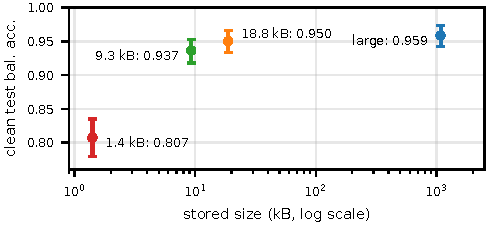
\includegraphics[width=\columnwidth]{fig_size.pdf}
  \caption{Clean-test balanced accuracy (95\% CI) against stored size.}
  \label{fig:size}
\end{figure}

Every model scores 0.5 to 1.1\,pp below its validation score, and all four catch 98.8 to 98.9\% of tumors. For
reference, the authors' CNN got a test accuracy of 0.847; my large model reaches 0.962, and even the 9.3\,kB
model 0.938. Without any pretraining, the large model came within 1 to 2\,pp of the fine-tuned ImageNet models
(0.971 and 0.983), and I was very impressed by the small models: the 18.8\,kB model is 57 times smaller and loses
only 0.9\,pp.

\section{Error analysis}
The models share errors far more often than chance (the large and 18.8\,kB models both miss 4 tumors where 0.1
would be expected), but most errors belong to one model: 11 of the 19 missed tumors are missed by only one. In
the images (Fig.~\ref{fig:errors}), the missed tumors are a mix of scan types and equipment, with contrast that
varies wildly from the rest of the set and zoom that is too close or too far, while the correctly detected tumors
have very similar contrast, layout and positioning. The false alarms show varying contrast, bad cropping,
irregular positioning and borders around the image. This is the scan-type shortcut from the data section showing
up: a tumor on an unusual scan looks like the mixed no-tumor class. The main remaining confusion is glioma vs
meningioma (12 of the large model's 34 errors).

\begin{figure}[t]
  \centering
  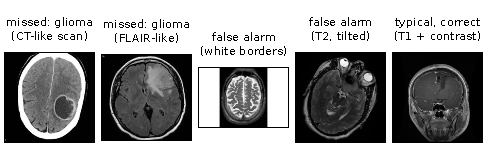
\includegraphics[width=\columnwidth]{fig_errors.pdf}
  \caption{Clean-test examples, as stored: tumors missed by at least one model, false alarms, and a typical
           correctly detected tumor.}
  \label{fig:errors}
\end{figure}

\section{Limitations and next steps}
Stronger input augmentation was tested and dropped, as it did not raise the validation score, but validation is
dominated by typical scans. A model expected to handle images with this much variation would most likely need
it, along with data from more scan types and sources. The large model should also be retrained with plain
cross-entropy instead of label smoothing, which gained only 0.03\,pp and most likely hurt distillation.

\small
\begin{thebibliography}{9}\setlength{\itemsep}{0pt}
\bibitem{data} M.\,I.\,K.\ Hira, M.\,S.\ Hossain, M.\,M.\,A.\ Bithee, U.\,S.\ Sara, M.\,M.\ Hasan, A.\,A.\ Towsif,
  M.\,K.\ Ahmed. \emph{BDNeuro-MRI: A Bangladeshi Clinical Brain Tumor MRI Dataset for Four-Class Deep Learning
  Classification}, v7. Mendeley Data, 2026. \url{https://doi.org/10.17632/zwr4ntf94j.7}
\bibitem{bench} Dataset authors' benchmark. \url{https://github.com/irfanulkabirhira/A-Bangladeshi-Clinical-Brain-Tumor-MRI-Dataset-for-Four-Class-Deep-Learning-Classification}
\bibitem{hinton} G.\ Hinton, O.\ Vinyals, J.\ Dean. Distilling the knowledge in a neural network.
  arXiv:1503.02531, 2015.
\bibitem{muller} R.\ Müller, S.\ Kornblith, G.\ Hinton. When does label smoothing help? NeurIPS, 2019.
\end{thebibliography}

\end{document}
